\chapter{}

{\textcolor{teal}{\section{User Story}}

\subsection{Use Case 1}
A student named Aporbo wants to communicate with a faculty for assist. He got two options 
i) Either he can search in the site for that particular faculty’s id to send text or \\
ii) He can post in groups to know how to be contacted with that faculty. \\
\subsection{Use Case 2}
A teacher has to discuss an urgent matter that should be noticed by the students immediately. \\
A) He/She can post in the group or \\
B)Send a text to each student separately\\ 
\subsection{Use Case 3}
Use Case 3:
Any club wants to advertise of their activities \\
A) Can announce in a group and share in other groups \\
B)Can send invitations to the faculties and students in their inboxes. \\

\subsection{Limitation of the Site }
• Can’t store the profiles or ids by adding in one’s profile or by following \\
• Lack of privacy that can violate the rules of the site. For example: sending messages unnecessarily to a faculty. \\
• Can’t communicate via call or send any voice records\\

\newpage
{\textcolor{teal}{\section{Solution Description}}}

\lipsum  % Remplacer avec votre texte
\subsection{Architecture }
Database will receive requests of students and faculties from multiple types such android,
iOS and windows apps and also browsers. There is mySQL for database system.
\begin{figure}[ht]
\includegraphics[width=10cm]{figures/figure1.jpg}
 
\label{fig:graph}
\end{figure}
\subsection{Front-end Plan }
User:\\
1. Login and register page\\
2. register steps page\\
3. Home page\\
4. Timeline\\
5. Help\\
6. profile\\
7. About\\
8. setings\\
a. Forgot Password\\
b. Profile Management\\
c.Deactivation account 
3. Searching profile:\\
a. Faculty search\\
b. Student Search\\

Admin:\\
1.login\\
2.all public post\\
3.help reply\\
4.all profiles\\
5.settings:\\
a.password changed\\
b.deactivate\\
6.Send notice\\
\lipsum % Remplacer avec votre texte
\subsection{Backend development}\\
1. Account Creating, Password Recover:\\
a. Sign up form.\\
b. Login\\
c. Forgot Password\\
2. Profile Management:\\
a.  Profile\\
d. Others\\
3. Searching facility:\\
a. Faculty search\\
b. Student Search\\
4.posts images\\
5.chats\\
6.notices\\
\lipsum  % Remplacer avec votre texte
\subsection{Tools and Technologies}

1. Database: Mysql\\
2. PHP\\
3.Javascript
4.html
5.css
\newpage
{\textcolor{teal}{\section{Advantage}}

\lipsum  % Remplacer avec votre texte
There are six major advantages of NSUBUD'S social networking site:
interoperability, accessibility, reusability, durability, maintenance ability, and adaptability, which in themselves constitute the concept of NSUBUDS.
1.NSUBUD'S supports content in the formats: text, image.\\
2. One can access posts anytime, from everywhere, anyone can modify and repost them, and others can see the updated post.\\
3. Students can approach any faculty to get help in their courses for better understand and also can get help from administration in their needs.\\
4. The NSUer, faculty, and administration staff can communicate thoroughly without any hassle and pass any information within a short period of time.\\
5. Students can learn and get information collaboratively by setting up a website with the NSUBUDS software and
helps Keeps organizations up-to-date with compliance
regulations. If your organization must stay up-to-date with current compliance regulations, then NSUBUDS can be an invaluable tool.\\


{\textcolor{teal}{\section{Hardware and Hosting Plan}}
Here is a list of possible cloud plans. We have to choose one that fits best and also economical.
\begin{figure}[ht]
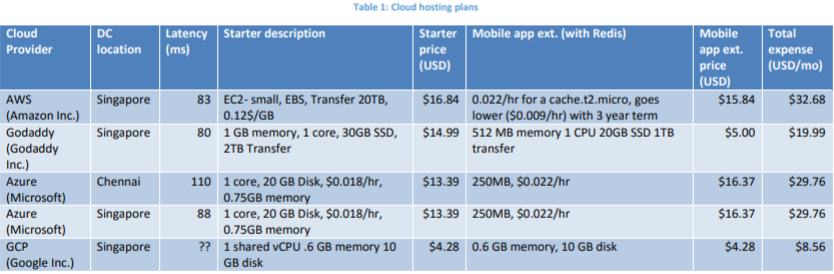
\includegraphics[width=18cm]{figures/table1.png}
 
\label{fig:graph}
\end{figure}

\newpage
{\textcolor{teal}{\section{Collaboration Plan}}
\begin{figure}[ht]
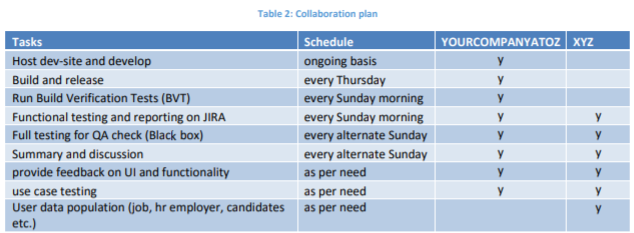
\includegraphics[width=18cm]{figures/table2.png}
 
\label{fig:graph}
\end{figure}

{\textcolor{teal}{\section{Project Schedule }}
Phase 1 will take a total of 6 weeks from the day of start. Calculated Man-month = 8.5/4 = 2.123. Excluding front end development it will become
\begin{figure}[ht]
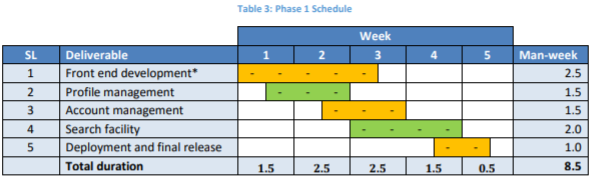
\includegraphics[width=18cm]{figures/table3.png}
 
\label{fig:graph}
\end{figure}